% -----------------------------------------  
% Autogenerated LaTeX file from XML DocBook  
% -----------------------------------------  
%%<params>
%%</params>
\documentclass[letterpaper,10pt,twoside,openright]{book}
\IfFileExists{ifxetex.sty}{%
    \usepackage{ifxetex}%
  }{%
    \newif\ifxetex
    \xetexfalse
  }
  \ifxetex
\usepackage{fontspec}
\usepackage{xltxtra}
\setmainfont{DejaVu Serif}
\setsansfont{DejaVu Sans}
\setmonofont{DejaVu Sans Mono}
\else
\usepackage[T1]{fontenc}
\usepackage[latin1]{inputenc}
\fi
\usepackage{fancybox}
\usepackage{makeidx}
\usepackage[hyperlink]{cll}
\renewcommand{\DBKreleaseinfo}{}
\renewcommand{\DBKrevhistory}{}
\setcounter{tocdepth}{5}
\setcounter{secnumdepth}{5}
\def\DBKcopyright{\noindent Copyright \textnormal{\copyright} Test Copyright Year 2014 Test Copyright Holder}


\def\DBKsubtitle{Test Subtitle}



\title{The Complete Lojban Language}
\author{AuthorFirstName AuthorSurName}
\hypersetup{%
pdfcreator={DBLaTeX-0.3.4},%
pdftitle={The Complete Lojban Language},%
pdfauthor={AuthorFirstName AuthorSurName}%
}
\renewcommand{\DBKindexation}{}
\makeindex
\makeglossary
\begin{document}
\lstsetup
\frontmatter
\maketitle
\tableofcontents
\mainmatter

% ------- 
% Chapter 
% ------- 

\chapter{COVERAGE: SMALL 1}
\label{chapter-tour}\hyperlabel{chapter-tour}%
    
\noindent\begin{minipage}[c]{\linewidth}
\begin{center}
\imgexists{media/chapter-tour.gif}{{\imgevalsize{media/chapter-tour.gif}{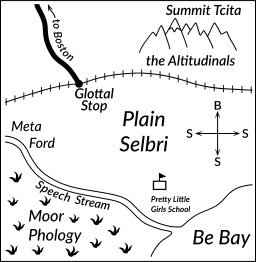
\includegraphics[width=\imgwidth,height=\imgheight,keepaspectratio=true]{media/chapter-tour.gif}}}}{}\end{center}
\end{minipage}

  
\section{The concept of the bridi}
\label{section-bridi}\hyperlabel{section-bridi}%
    
 \index{bridi!concept of} This chapter gives diagrammed examples of basic Lojban sentence structures. The most general pattern is covered first, followed by successive variations on the basic components of the Lojban sentence. There are many more capabilities not covered in this chapter, but covered in detail in later chapters, so this chapter is a 
 “quick tour” of the material later covered more slowly throughout the book. It also introduces most of the Lojban words used to discuss Lojban grammar.
  
         Let us consider John and Sam and three statements about them:
   
\begin{longfloat}{example}{\caption[{    }]{  \index{father!example}  \index{John and Sam!example}   \label{c2e1d1}\hyperlabel{c2e1d1}  }
\label{example-random-id-qIuj}\hyperlabel{example-random-id-qIuj}%
}

John is the father of Sam.

\end{longfloat}
  
 \index{sumti!relation with bridi} \index{brivla!relation to bridi} \index{predication!compared with bridi} \index{bridi!compared with predication} \index{predication!as a relationship} \index{relationship!active/static/attributive compared} These examples all describe relationships between John and Sam. However, in English, we use the noun 
  “father” to describe a static relationship in 
 Example \ref{example-random-id-qIuj}, the verb 
 “hits” to describe an active relationship in 
      In formal logic this whole structure is called a
 “predication”; in Lojban it is called a
 \hyperlink{valsi-bridi}{\emph{\emph{\index{bridi}bridi}}}, and the central part of speech is the
 \hyperlink{valsi-selbri}{\emph{\emph{\index{selbri}selbri}}}. 
 
    % --------	
% GLOSSARY	
% --------	

\chapter{Lojban Word Glossary}

All definitions in this glossary are brief and unofficial.
Only the published dictionary is a truly official reference for word
definitions.  These definitions are here simply as a quick reference.


\section*{B}

\noindent
\begin{description}
\item[\hypertarget{valsi-bridi}{bridi}]~ 

x$_{\text{1}}$ (text) is a predicate relationship with relation x$_{\text{2}}$ among arguments (sequence/set) x$_{\text{3}}$.



\end{description}

\section*{S}

\noindent
\begin{description}
\item[\hypertarget{valsi-selbri}{selbri}]~ 

NO JBOVLASTE DEFINITION FOR "selbri" FOUND!



\end{description}
\printindex

\end{document}
